\documentclass[conference]{IEEEtran}
\usepackage{cite}
\usepackage{amsmath,amssymb,amsfonts}
\usepackage{algorithmic}
\usepackage{graphicx}
\usepackage{subcaption}
\usepackage{textcomp}
\usepackage{xcolor}
\usepackage{amsmath}
\def\BibTeX{{\rm B\kern-.05em{\sc i\kern-.025em b}\kern-.08em
    T\kern-.1667em\lower.7ex\hbox{E}\kern-.125emX}}
\begin{document}

\title{Decentralized Protocol for Poly Queer Matchmaking}

\author{\IEEEauthorblockN{Silly Peter}
\IEEEauthorblockA{\textit{Kinky Bitch} \\
ORCID: 0420-6969-0666-8008}
}

\maketitle

\begin{abstract}
Proposes a decentralized protocol for verifying mutual sexual interest within a group. Pairs of individuals know who they want to fuck, learn who also wants to fuck them back, but don't learn any information about other sexual interests (ie. one sided desires to fuck not originating from them). Describes two physical solutions and one digital solution with varying requirements and pros/cons.
\end{abstract}

\begin{IEEEkeywords}
decentralized, mutual interest, queer fuckery
\end{IEEEkeywords}

\section{Introduction of the Problem}
When deciding to match-make a group of individuals, the problem is traditionally pairing heterosexual, monogamous individuals with their preferred person and where every person needs to be paired. Historically this has been solved by a central authority that knows each party's preferences and this authority does its best to pair each person with a suitable match (minimizing some loss heuristic). This problem is dramatically different with a group where the parties are queer, where polyamory is the norm, not everybody needs to be matched, and where having a central authority can be problematic. The problem is no longer a 1-to-1 pairing problem, but a many-to-many pairing problem. More specifically, parties need a mechanism for validating shared mutual interest. Since this interest, in the situation that inspired this paper, is primarily sexual, it shall be phrased as “Intention(s) To Fuck” (or ITF) for the intention of some party A towards some party B regardless of reciprocity, and “Mutual Intention(s) To Fuck” (or MITF) if and only if there exists an ITF from party A to party B and another IFT from party B to party A. ITF can’t be from party A to the same party A.

This situation can also be defined as a directed graph: 
\begin{align*}
& G=(V, A)\\
& V = \text{the set of all parties involved} \\
& A = \{(x,y)\; \forall x,y \in V \: s.t.\: x \neq y \: \exists ITF (x \rightarrow y)\}
\end{align*}

The goal of this protocol is to then inform each party of MITF they are involved in, but give no information about ITF they are not involved in and not the originator of. Each party starts knowing ITF originating from themselves (edges starting at their vertex) and all vertices, but nothing else.


\section{Reasons for a Decentralized Protocol}
Aside from general distaste in trusting central authority, dedicating a party to be a central authority would remove them from the matchmaking process. Even if they could be trusted to act fairly despite having knowledge of all ITF (especially those directed at themselves), other parties couldn’t submit an ITF to the matchmaker and have the same secrecy promised to other interactions. For example, if party A is the matchmaker and party B submits an ITF (b $\rightarrow$ a) to A, A knows that B had an ITF without that ITF needing to be reciprocated (knowledge of more than just MITF involving self).

In practice, this means a group needs to dedicate an outside party as the matchmaker. An outside party won’t be trusted/known by all inside parties as much as an inside party would be. The group then has to decide if an internal party is excluded, or if an external party with less trust is used. Both options are sub-optimal.


\section{High Level of Proposed Solution 1}
This protocol happens in 2 rounds. For round 1, each party that wishes to participate generates globally unique secrets and associates each with an ITF (self $\rightarrow$ other). For each ITF (self $\rightarrow$ other), a party communicates the associated secret in some discrete fashion to the “other” party. For round 2, for each ITF (self → other) a party communicates all their received secrets discretely to the “other” party. Each party can then check if they received any of their initial unique secrets. Since these are associated with a single ITF, the party can determine which ITF is now a MITF. Each party knows their ITF, MITF they are involved in, and random data from the other ITF sent to them in round 2.

The concrete implementations solve the following problems in their own ways:
\begin{itemize}
\item globally unique secret generation
\item discrete message passing
\item limiting useful information gained from random data/metadata from round 2
\end{itemize}

\section{Physical Implementation of Method 1}

\subsection{Requirements}\label{AA}
This protocol requires N parties, deck(s) of cards, writing materials, index cards, and N opaque containers. To accommodate M total ITF, there must be M unique playing cards for the simple approach or M*N unique playing cards for the nice approach. This can also be formulated using the max ITF per party as m. The protocol would then require m*N unique playing cards (worst case) for the simple approach or m*N*N (worst case) for the nice approach. The index cards required will also be equal to the total number of ITF.

In summary, if N = number of parties, M = number of ITF:
\begin{itemize}
\item N opaque containers
\item M*N playing cards
\item M index cards
\end{itemize}

\subsection{Simple Approach}
Each party claims a container as their own. This claim is public (all parties know claims) and unique (no 2 parties can claim the same container).

For round 1, each party draws cards randomly for each ITF they have (self $\rightarrow$ other). The party secretly memorizes/writes down the cards they have drawn and the ITF associated with that card. One at a time, the parties place their drawn cards into the container of the “other” person (self $\rightarrow$ other) of the associated ITF. This should be done with only one party in the room/line of sight of the containers at a time to allow discrete message passing.
For round 2, each party secretly reads the cards in their container. They then write down all the card values (as much information needed to be globally unique) on index cards (equal to the number of their ITF). These identical index cards are then discreetly placed in the “other” container for every ITF (self $\rightarrow$ other).

When all parties read the contents of their containers at the end of round 2, they should have index cards with unique values on them. If any of these unique values match their initial unique values, a party knows the associated ITF is a MITF.

\subsection{Limitations of the Simple Approach}
The problem with this approach is the index cards received in round 2 contain information about the quantity of ITF sent to the now identified party. If the unique value X is associated with ITF (self $\rightarrow$ B), the index card containing X is known to be B’s, therefore the number of unique values on that card is the number of ITF (any $\rightarrow$ B). Parties also know the number of ITF (any $\rightarrow$ self), which can be discouraging if this number is low, especially if it is lower than other parties' number of ITF.

\subsection{Nice Approach}
This modifies the simple approach in round 1. Instead of each party only drawing cards equal to the number of ITF they have (self $\rightarrow$ other), they draw N cards total. Only some of those cards is associated with an ITF, the other cards are dummy cards and are forgotten by the party that drew them. When placing cards in the desired containers, only the associated value is placed in the “other” container for that ITF (self $\rightarrow$ other). The dummy cards are placed in every container there wasn't an ITF for (self $\rightarrow$ dummy). The dummy values are still sent in round 2, but since they've been forgotten the values don't communicate information.

Another key part of round 2 here is the creation of dummy sets. Each party will receive N-1 cards in round 1. To create a dummy set, A takes N-1 new dummy cards and makes this the dummy set. For each other party A does not have an ITF (A $\rightarrow$ other), this dummy set is sent. The real set is sent to real connections just as in the normal protocol.

This leads to each container having the same number of cards in it. No single party can distinguish real cards versus dummy cards. A party then doesn’t gain information on the true number of ITF directed at themselves or at others. They also have the same amount of card sets, which also does not reveal how many true ITF were directed at themselves.



\section{Digital Implementation of Method 1}
\subsection{Requirements}
Each participating party needs a known public key, and an associated secret private key. All parties need an established central “dropping” message area where messages can be publicly placed and read by all parties. There also needs to be some mechanism of communicating consensus for the ends of round 1 and round 2.

\subsection{Protocol}
Each party randomly generates private secrets that are long enough to ensure uniqueness within the system. Each of these values are associated uniquely with an ITF (self $\rightarrow$ other).

For round 1, for each ITF (self $\rightarrow$ other) a user will encrypt the secret along with some publicly known magic bytes using the “other” party’s public key. These encrypted messages are then publicly placed in the message dropping area. Once all parties have finished dropping messages, all messages are read and decrypted individually by each party with their own private key. If the message contains the magic bytes, the message is known to be intended for them (ie. decryption success). The party then has discretely received the unique secret.

For round 2, each user does the same as in the physical protocol. All successfully received secrets are discretely passed to all “other” users for each ITF (self $\rightarrow$ other). Once all messages are dropped, all parties again decrypt all messages and check for the magic bytes.

\subsection{Limitations and Extension}
The modifications that are in the physical implementation’s nice version also work here to solve the same problems.


\section{Physical Implementation of Method 2}
This protocol, courage by proxy, differs from the above protocols but solves the same problem in a decentralized way. The requirements are also different.

\subsection{Requirements}
This requires N participating parties, N proxy parties, N index cards, and writing materials.

\subsection{Protocol}
The participating parties isolate themselves from the proxy parties.

For round 1, the participating group uniquely and publicly (within the group) assigns numbers to each party in the group. Individuals secretly write down their own number on the top of their index card and the number of the “other” party for each ITF (self $\rightarrow$ other) they have. These index cards are passed discretely off to the proxy parties. This can be done by placing them face down and having the proxy parties grab one each. Each proxy party will have 1 index card. The proxy parties isolate themselves from the participating parties.

For round 2, the proxy group shares their number (from the top of the index card) and represents that number. Each proxy party approaches each party that represents a number on their index card. If both parties have the other on their list, both mark so on the index card. Once all the parties have gone through their lists, the index cards are handed back to the participating party that owns that card. This can be done by laying them face down, sorted by number, and the participating party grabs their own.

In the end, all participating parties know the number (and therefore associated participating party) for all MITF. The proxy parties know how many ITF and MITF a random participating party has, but not the associated participating party.


\section{Examples of Method 1}
The graphs on the following page demonstrate various examples of Method 1 in action.


\begin{figure*}[h!]
\centering
\setkeys{Gin}{width=0.31\linewidth,height=10cm}
\subfloat [No mutual edges. \label{fig:g1}]{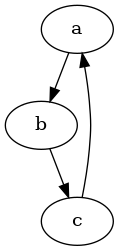
\includegraphics{figure1.png} }
\subfloat [One mutual edge. \label{fig:g2}]{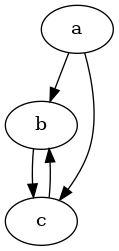
\includegraphics{figure2.png} }
\subfloat [Two mutual edges. \label{fig:g3}]{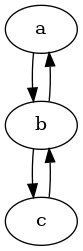
\includegraphics{figure3.png} }

\caption{Example Graphs}
\end{figure*}


\subsection{Running on Graph A}
For figure 1, each party has only 1 ITF each. Each party would have the following secrets associated with their ITF:
\begin{itemize}
\item A : \{0 : (A$\rightarrow$B)\}
\item B : \{1 : (B$\rightarrow$C)\}
\item C : \{2 : (C$\rightarrow$A)\}
\end{itemize}

Round 1 gives each party the following messages:
\begin{itemize}
\item A : \{2\}
\item B : \{0\}
\item C : \{1\}
\end{itemize}

Round 2 gives each party the following messages:
\begin{itemize}
\item A : \{1\}
\item B : \{2\}
\item C : \{0\}
\end{itemize}

Since nobody has their initial secret, no MITF exist.

\subsection{Running on Graph B}
For setup, these are the secrets and associated ITF:
\begin{itemize}
\item A : \{0 : (A$\rightarrow$B), 1 : (A$\rightarrow$C)\}
\item B : \{2 : (B$\rightarrow$C)\}
\item C : \{3 : (C$\rightarrow$B)\}
\end{itemize}

Round 1 gives each party the following messages:
\begin{itemize}
\item A : $\emptyset$
\item B : \{0, 3\}
\item C : \{1, 2\}
\end{itemize}

Round 2 gives each party the following messages:
\begin{itemize}
\item A : $\emptyset$
\item B : \{\{1, 2\}\}
\item C : \{\{0, 3\}\}
\end{itemize}

A received nothing, meaning there are no MITF involving A. B received 2, meaning the ITF (B$\rightarrow$C) is a MITF. C received 4, meaning the ITF (C$\rightarrow$B) is a MITF.

\subsection{Running on Graph C}
For setup, these are the secrets and associated ITF:
\begin{itemize}
\item A : \{0 : (A$\rightarrow$B)\}
\item B : \{1 : (B$\rightarrow$A), 2 : (B$\rightarrow$C)\}
\item C : \{3 : (C$\rightarrow$B)\}
\end{itemize}

Round 1 gives each party the following messages:
\begin{itemize}
\item A : \{1\}
\item B : \{0, 3\}
\item C : \{2\}
\end{itemize}

Round 2 gives each party the following messages:
\begin{itemize}
\item A : \{\{0, 3\}\}
\item B : \{\{1\}, \{2\}\}
\item C : \{\{0, 3\}\}
\end{itemize}

A received 0, meaning the ITF (A$\rightarrow$B) is a MITF. B received 1, meaning the ITF (B$\rightarrow$A) is a MITF. B also received 2, meaning the ITF (B$\rightarrow$C) is a MITF. C received 3, meaning the ITF (C$\rightarrow$B) is a MITF.

\subsection{Running the Nice modification on Graph B}
For setup, these are the secrets and associated IFT. Dummy values are indicated as secrets with no ITF:
\begin{itemize}
\item A : \{0 : (A$\rightarrow$B), 1 : (A$\rightarrow$C)\}
\item B : \{2 : (B$\rightarrow$C), 3\}
\item C : \{4 : (C$\rightarrow$B), 5\}
\end{itemize}

Round 1 gives each party the following messages:
\begin{itemize}
\item A : \{3, 5\}
\item B : \{0, 4\}
\item C : \{1, 2\}
\end{itemize}

Round 2 gives each party the following messages. The dummy sets created here are \{6,7\} and \{8,9\}:
\begin{itemize}
\item A : \{\{6,7\}, \{8,9\}\}
\item B : \{\{3,5\}, \{1,2\}\}
\item C : \{\{3,5\}, \{0,4\}\}
\end{itemize}

A received 6, 7, 8 and 9, but none are A's remembered values meaning there were no MITF involving A. B received 1, 2, 3, and 5, and 2 was the only remembered value so B knows (B$\rightarrow$C) is a MITF. C received 0, 3, 4 and 5, and 4 was the only remembered value so C knows (C$\rightarrow$C) is a MITF.

The dummy values are forgotten after sending, so they can't leak information about other connections. Each party ended up with the same number of number sets, so no party knows how many people genuinely had ITF directed at them.

\end{document}
